

\documentclass{article}
\usepackage[utf8]{inputenc}
\usepackage[utf8]{inputenc}
\usepackage[T1]{fontenc}
\usepackage[english]{babel}
\usepackage{fullpage}
\usepackage{color}
\usepackage[table]{xcolor}
\usepackage{listings}
 
\definecolor{darkWhite}{rgb}{0.94,0.94,0.94}
 
\lstset{
  aboveskip=3mm,
  belowskip=-2mm,
  backgroundcolor=\color{darkWhite},
  basicstyle=\footnotesize,
  breakatwhitespace=false,
  breaklines=true,
  captionpos=b,
  commentstyle=\color{red},
  deletekeywords={...},
  escapeinside={\%*}{*)},
  extendedchars=true,
  framexleftmargin=16pt,
  framextopmargin=3pt,
  framexbottommargin=6pt,
  frame=tb,
  keepspaces=true,
  keywordstyle=\color{blue},
  language=C,
  literate=
  {²}{{\textsuperscript{2}}}1
  {⁴}{{\textsuperscript{4}}}1
  {⁶}{{\textsuperscript{6}}}1
  {⁸}{{\textsuperscript{8}}}1
  {€}{{\euro{}}}1
  {é}{{\'e}}1
  {è}{{\`{e}}}1
  {ê}{{\^{e}}}1
  {ë}{{\¨{e}}}1
  {É}{{\'{E}}}1
  {Ê}{{\^{E}}}1
  {û}{{\^{u}}}1
  {ù}{{\`{u}}}1
  {â}{{\^{a}}}1
  {à}{{\`{a}}}1
  {á}{{\'{a}}}1
  {ã}{{\~{a}}}1
  {Á}{{\'{A}}}1
  {Â}{{\^{A}}}1
  {Ã}{{\~{A}}}1
  {ç}{{\c{c}}}1
  {Ç}{{\c{C}}}1
  {õ}{{\~{o}}}1
  {ó}{{\'{o}}}1
  {ô}{{\^{o}}}1
  {Õ}{{\~{O}}}1
  {Ó}{{\'{O}}}1
  {Ô}{{\^{O}}}1
  {î}{{\^{i}}}1
  {Î}{{\^{I}}}1
  {í}{{\'{i}}}1
  {Í}{{\~{Í}}}1,
  morekeywords={*,...},
  numbers=left,
  numbersep=10pt,
  numberstyle=\tiny\color{black},
  rulecolor=\color{black},
  showspaces=false,
  showstringspaces=false,
  showtabs=false,
  stepnumber=1,
  stringstyle=\color{gray},
  tabsize=4,
  title=\lstname,
}
\usepackage{graphicx}
\graphicspath{ {./images/} }
\title{HAI804I – Analyse et Traitement d'Images}
\author{Fabien Caballero }

\begin{document}  

\maketitle
    \tableofcontents

\newpage

\section{Création d'une image en niveaux de gris}
Pour transformer une image couleur en niveau de gris on récupère la composante Y de l'espace YCrCb et on en fait une image pgm.
Il faut pour chaque pixel récupérer un certain coefficient de la composante rouge, un autre de la verte et un autre de la bleue du même pixel en couleur.

\begin{figure}[h!]
\centerline{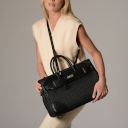
\includegraphics[scale=1.]{./rendus/sac.png}}
\caption{Image d'origine en couleur}

\qquad

\centerline{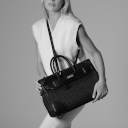
\includegraphics[scale=1.]{./rendus/sacgris.png}}
\caption{Image transformée en niveaux de gris}
\end{figure}

\begin{figure}[h!]
\centerline{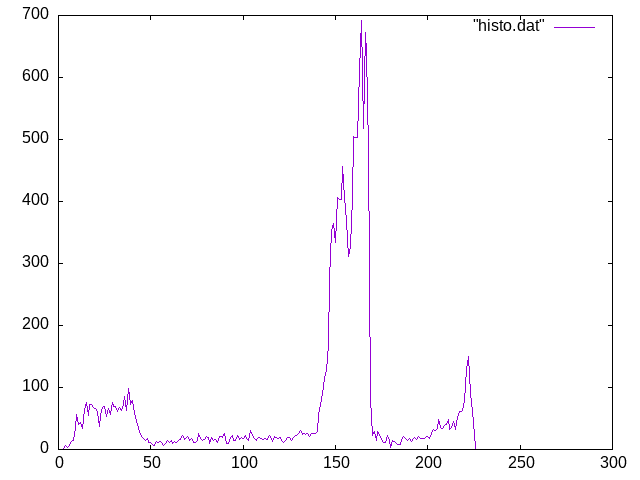
\includegraphics[scale=0.5]{./rendus/histogris.png}}
\caption{histogramme de l'image en niveaux de gris}

\end{figure}

\newpage
\section{Seuillage de l'histogramme}
\begin{lstlisting}
   OCTET *ImgOut;
    allocation_tableau(ImgOut, OCTET, nTaille);

    // 1 seuil
    for (int j = 0; j < nTaille; j++)
    {
        if (ImgIn[j] < s1)
            ImgOut[j] = 0;
        else
            ImgOut[j] = 255;
    }
\end{lstlisting}
En regardant l'histogramme j'ai choisi un seuil de 50 qui laissait apparaître seulement le sac en noir et tout le reste était blanc
\begin{figure}[h!]
\centerline{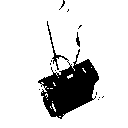
\includegraphics[scale=1.2]{./rendus/sacSeuil.png}}
\caption{image seuillée }
\end{figure}

\newpage
\section{Floutage d'image couleur}
Pour flouter il faut pour chaque pixel de l'image de sortie lui attribuer la moyenne des pixels voisins (lui compris).
\begin{lstlisting}
   int nTaille = nW * nH;
    OCTET *R, *G, *B, *Rf, *Gf, *Bf, *ImgOut;
    allocation_tableau(R, OCTET, nTaille);
    allocation_tableau(G, OCTET, nTaille);
    allocation_tableau(B, OCTET, nTaille);
    allocation_tableau(Rf, OCTET, nTaille);
    allocation_tableau(Gf, OCTET, nTaille);
    allocation_tableau(Bf, OCTET, nTaille);

    allocation_tableau(ImgOut, OCTET, nTaille * 3);
    planR(R, ImgIn, nTaille);
    planV(G, ImgIn, nTaille);
    planB(B, ImgIn, nTaille);

    for (int i = 0; i < nTaille; i++)
    {
        Rf[i] = R[i];
        Gf[i] = G[i];
        Bf[i] = B[i];
    }

    for (int i = 1; i < nH - 1; i++)
    {
        for (int j = 1; j < nW - 1; j++)
        {
            int somR =
                R[(i - 1) * nW + j - 1] + R[(i - 1) * nW + j] + R[(i - 1) * nW + j + 1] + R[i * nW + j - 1] + R[i * nW + j] + R[i * nW + j + 1] + R[(i + 1) * nW + j - 1] + R[(i + 1) * nW + j] + R[(i + 1) * nW + j + 1];

            Rf[i * nW + j] = somR / 9;

            int somG =
                G[(i - 1) * nW + j - 1] + G[(i - 1) * nW + j] + G[(i - 1) * nW + j + 1] + G[i * nW + j - 1] + G[i * nW + j] + G[i * nW + j + 1] + G[(i + 1) * nW + j - 1] + G[(i + 1) * nW + j] + G[(i + 1) * nW + j + 1];

            Gf[i * nW + j] = somG / 9;

            int somB =
                B[(i - 1) * nW + j - 1] + B[(i - 1) * nW + j] + B[(i - 1) * nW + j + 1] + B[i * nW + j - 1] + B[i * nW + j] + B[i * nW + j + 1] + B[(i + 1) * nW + j - 1] + B[(i + 1) * nW + j] + B[(i + 1) * nW + j + 1];

            Bf[i * nW + j] = somB / 9;
        }
    }

    for (int i = 0; i < nTaille; i++)
    {
        ImgOut[3 * i] = Rf[i];
        ImgOut[3 * i + 1] = Gf[i];
        ImgOut[3 * i + 2] = Bf[i];
    }

\end{lstlisting}
\begin{figure}[h!]
\centerline{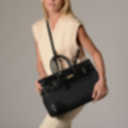
\includegraphics[scale=1.2]{./rendus/coulFlou.png}}
\caption{image couleur floue }
\end{figure}

\newpage
\section{Floutage du fond de l’image couleur}

Pour flouter que le fond on parcours tout les pixels (compteur i variant de 0 à w*h), pour chaque pixel de l'image seuillée (couleur binaire) on regarde si celui-ci est noir on définit la couleur du pixel de sortie de la même couleur que celui de l'image originale, car il appartient à l'objet (vu qu'il s'agit d'une image couleur il faut faire i*3, i*3+1 et i*3+2 pour toutes les images couleurs).
Et si le pixel est blanc on fait pareil mais en prenant la couleur de l'image floutée. 
\begin{lstlisting}
   for (size_t i = 0; i < ntaille; i++)
    {

        if (ImgSeuil[i] == 255)
        {
            ImgOut[i * 3] = ImgFlou[i * 3];
            ImgOut[i * 3 + 1] = ImgFlou[i * 3 + 1];
            ImgOut[i * 3 + 2] = ImgFlou[i * 3 + 2];
        }
        else
        {
            ImgOut[i * 3] = ImgIn[i * 3];
            ImgOut[i * 3 + 1] = ImgIn[i * 3 + 1];
            ImgOut[i * 3 + 2] = ImgIn[i * 3 + 2];
        }
    }

\end{lstlisting}

\begin{figure}[h!]
\centerline{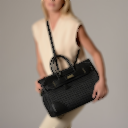
\includegraphics[scale=1.2]{./rendus/couleurFondFlou.png}}
\caption{image couleur avec fond flouté uniquement }
\end{figure}

\newpage
\section{Erosion et dilatation}

En appliquant erosion et dilatation, déja implémentée dans les tp précédents, on obtient une image seuillée avec quelques trous comblés.

\begin{figure}[h!]
\centerline{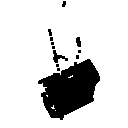
\includegraphics[scale=1.2]{./rendus/seuilEroDila.png}}
\caption{image seuillée érodée puis dilatée }
\end{figure}


Et lors du floutage du fond on remarque que l'objet est moins floutée sur certains endroits ou il l'était encore en utilisant l'image de seuil précédente.
\begin{figure}[h!]
\centerline{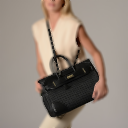
\includegraphics[scale=1.2]{./rendus/floufonderodila.png}}
\caption{image couleur avec fond flou à partir de l'image seuil précédente}
\end{figure}

\newpage
\section{Tracé d’une courbe ROC (receiver operating characteristic) et
calcul d’un F1 score}

Pour obtenir cette courbe on seuille notre image avec plusieurs valeurs (de 0 à 255), pour chaque image seuillée avec un seuil on calcul le nombre de vrais positifs, de faux positifs, de vrai négatifs et de faux négatifs.
Puis dans un fichier ROC.dat on met en x, 1- la spécificité (1-(VN/(VN/FP))) et en y la sensibilité (VP/(VP+FN)).
On fait ça pour chaque valeurs de seuils, on obtient donc à la fin 256 tuples (x,y) et on trace notre courbe avec gnuplot. 
\begin{figure}[h!]
\centerline{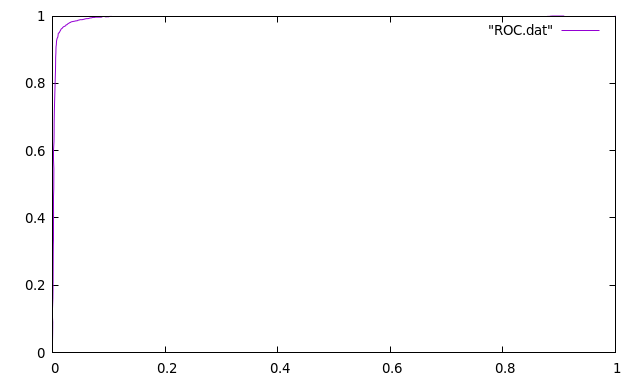
\includegraphics[scale=0.6]{./rendus/ROC.png}}
\caption{courbe ROC}
\end{figure}

On cherche ensuite la valeur de seuil qui minimise FP et FN pour cela on utilise l'indice de Youden.
Cela consiste à prendre, pour chaque pixel, FP+FN-1 et prendre le max de tout les FP+FN-1.
On obtient donc le seuil optimal, on récupère pour ce seuil la valeur de vrais positifs, de faux positifs et de faux négatifs.
On peut grâce à ces valeurs calculer la précision (TP/(TP+FN)), le rappel (TP/TP+FN) et le F1-score (2*precision*rappel/(precision+rappel)).
La précision correspond au taux de vrais positifs sur l'ensemble des positifs trouvés (pas d'unité ou poucentage), le rappel (pas d'unité ou poucentage) correspond au taux de vrais positifs sur par rapport à tout les positifs réels.

\textbf{\\\\Precision : 0.858349 \\\\ Rappel : 0.977434 \\\\ F1 Score : 0.914029}




\end{document}